\section{Metrics}
		
	\normalsize
	{
		The Metrics provided is a static analysis of the code.  The gathering of statistics such as inheritance depth, lines of code, 
		number of classes etc.  The estimation of complexity and maintainability is computed from this information with the goal of 
		determining the quality of the software.  
		\newline
		\newline
		The study of code metrics can help identify potential issues in large software projects.
		The resulting identification of trouble spots and the re-engineering can help to support the software evolution and the
		improvement of software process improvement (SPI) techniques.

		\vspace{1mm}
		\subsection{Static Analysis Tools}
		There are multiple tools and plug-ins available to achieve a static code analysis.  Three tools were chosen as each provided
		different types of measurements for the analysis. 
		
		\vspace{1mm}
				
		\begin{itemize}
			\item \textbf{Visual Studio}
				\begin{itemize}
					\item provides minimal metrics including, lines of code, maintainability index, cyclomatic complexity and class coupling
				\end{itemize}
				
			\item \textbf{Campwood Software LLC SourceMonitor}
				\begin{itemize}
					\item focuses on method analysis such as documentation, minimum/maximum average complexity and nesting levels
				\end{itemize}	
									
			\item \textbf{NDepend}
				\begin{itemize}
					\item focuses more on quality attributes such as coupling and dependency management
				\end{itemize}
				
			\item \textbf{JetBrains DotCover}
				\begin{itemize}
					\item was used for code coverage analysis.
				\end{itemize}	
		\end{itemize}
					
		As each tool implements their analysis slightly differently resulting in different metrics, 
		the choice for three tools was obvious in gaining a more comprehensive overview.  
		Some vendors choose either Mccabe metrics or Halstead Metrics 
		and may also add additional vendor massaging eg. Logarithmic scales.  
		The tool used will be identified for each metric presented.	
		\newline		
	}	
		
		
%%%%%%%%%%%%%%%%%%%%%%%%%%%%%%%%%%%%%%%%%%%%%%%%%%%%%%%%%%%%%%%%%%%
%%%%%%%%%%%%%%%%%%%%%%%%%%%%%%%%%%%%%%%%%%%%%%%%%%%%%%%%%%%%%%%%%%%	
			
\newpage
			
	\subsection{Maintainability Index}
				
		\vspace{-5mm}
		\textit
		{
			\begin{itemize}
				\item \textbf{Maintainability Index}
					\begin{itemize}
						\item Calculates an index value between 0 and 100 that represents the relative ease of maintaining the code
						\item A high value means better maintainability
						\item A green rating is between 20 and 100 and indicates that the code has good maintainability 
						\item A yellow rating is between 10 and 19 and indicates that the code is moderately maintainable
						\item A red rating is between 0 and 9 and indicates low maintainability 
					\end{itemize}
			\end{itemize}
		} 
		-- \citet{MicroSoftMetrics} 
		\vspace{5mm}
		
		\large{\bfseries{Interpretation}}
		\vspace{2mm}
		
		\normalsize
		Microsoft here use qualitative terms to define the maintainability index, in more scientific or quantitative terms, the formula
		for this is shown in Fig. \ref{fig:MaintainabilityIndexForumla}.
		
		\begin{multicols}{2}
		
			\vspace{25mm}
			Maurice Howard Halstead introduced the 'Halstead complexity measures' in 1977 as a means of establishing an empirical science for software development. 
			A further analysis of this theory is outside the scope of this paper and i will ask the reader to refer to the reference. (\citet{Halstead})
			\newline
			\newline

			\large{\bfseries{Analysis \& Improvement}}
			\newline
			\normalsize					
			There is not much we can tell from this information other than the size may indicate maintainability and understandability problems.
			\newline
			\newline
			During the calculation of these metrics the blank lines of code were left out by source monitor, contrary to the definition.  
			For the C\# analysis the larger of the two indicators 44,996, includes generated designer files generated by visual studio, but modified during development.
			\newline
			
		\columnbreak

		\vspace{-15mm}
		\begin{figurehere}
			\inputminted[linenos=true,fontsize=\footnotesize,tabsize=2,xleftmargin=1cm]{csharp}{pages/chapter4/smippets/mi.txt}
			\vspace{-5mm}
			\caption{Maintainability Index Formula}
			\label{fig:MaintainabilityIndexForumla}
		\end{figurehere}		

		\vspace{5mm}			
		\begin{figurehere}
			\centering
			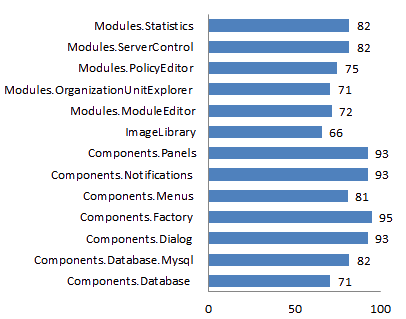
\includegraphics[scale=0.75]{pages/chapter4/figures/maintainability.png}
			\vspace{-5mm}
			\caption{Maintainability index}
			\label{fig:MaintainabilityIndex}
		\end{figurehere}	
		
	\end{multicols}	
		
%%%%%%%%%%%%%%%%%%%%%%%%%%%%%%%%%%%%%%%%%%%%%%%%%%%%%%%%%%%%%%%%%%%
%%%%%%%%%%%%%%%%%%%%%%%%%%%%%%%%%%%%%%%%%%%%%%%%%%%%%%%%%%%%%%%%%%%	

\newpage
	
	\subsection{Cyclomatic Complexity}
	
		\vspace{-7mm}
		\textit
		{
			\begin{itemize}
				\item \textbf{Cyclomatic Complexity}
					\begin{itemize}
						\item Measures the structural complexity of the code
						\item It is created by calculating the number of different code paths in the flow of the program
						\item A program that has complex control flow will require more tests to achieve good code coverage and will be less maintainable
					\end{itemize}	
			\end{itemize}
		} 
		-- \citet{MicroSoftMetrics} 
		\newline							
		
		\vspace{-3mm}
		\large{\bfseries{Interpretation}}
		\vspace{1mm}
		
		\normalsize
		{
			This measures the total number of individual paths or block levels through the code. 
			This is calculated by counting the number of decision points such as if, switch, while, foreach and for loops statements. 
			This measurement is a good indication on the number of unit tests and resulting code coverage. Lower is better.		
			It can also indicate the complexity of the test cases which would be as complex as the code itself.				
			\begin{center}
				cyclomatic complexity = edges - nodes + 1
			\end{center}
			\vspace{3mm}
			In this formula the nodes represent logic branches and an edge represents the path between nodes.
			The rule calculation reports a possible problem when the cyclomatic complexity is greater than 25.
			\newline	
		}			
			
		\vspace{-9mm}
		\begin{multicols}{2}

			\large{\bfseries{Analysis \& Improvement}}
			\vspace{1mm}

			\normalsize
			{
				From face value the cyclomatic index seems rather high for some of the dynamic link libraries. 
				These values however are based upon all the files that are encapsulated within the dynamic link libraries, 
				including structs and classes.
				\newline
				\newline
				The factory dynamic link library which is the most complex encapsulates 18 classes   
				and has an average complexity of 30 (545 complexity/18 classes).
				\newline
				\newline
				Although slightly over the recommended limit of 25, i don't believe that this is cause for concern as there is a degree 
				of complexity associated with composite, pluggable or modular architectures as indicated by the analysis of Microsoft Prism
				composite library in Fig. \ref{fig:MicrosoftPrismBestPracticesMetric}.
				\newline
				In section \ref{sec:linspreadresult} (line spread) we can see the average complexity for the
				entire product is approximately 15.  This figure is well within the recommended 25 limit. 
				\newline
				\newline
			}				
					
			\begin{figurehere}
				\centering
				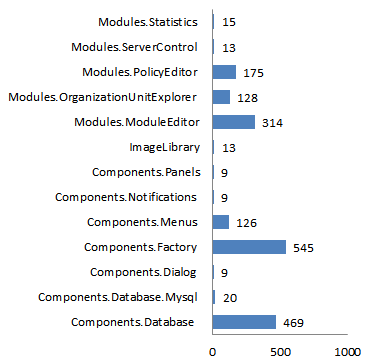
\includegraphics[scale=0.9]{pages/chapter4/figures/complex.png}
				\vspace{-5mm}
				\caption{Cyclomatic Complexity}
				\label{fig:CyclomaticComplexity}
			\end{figurehere}
		
			\vspace{5mm}
			\begin{figurehere}
				\centering
				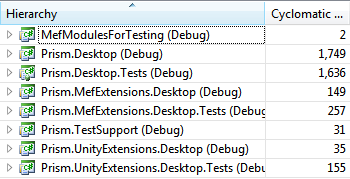
\includegraphics[scale=0.7]{pages/chapter4/figures/prismcomplex.png}
				\caption{Microsoft Prism - Best Practices Metric}
				\label{fig:MicrosoftPrismBestPracticesMetric}
			\end{figurehere}	
		
		\end{multicols}

%%%%%%%%%%%%%%%%%%%%%%%%%%%%%%%%%%%%%%%%%%%%%%%%%%%%%%%%%%%%%%%%%%%
%%%%%%%%%%%%%%%%%%%%%%%%%%%%%%%%%%%%%%%%%%%%%%%%%%%%%%%%%%%%%%%%%%%	

	\vspace{-6mm}
	\subsection{Depth Of Inheritance}
			
		\vspace{-8mm}
		\textit
		{
			\begin{itemize}
				\item \textbf{Depth of Inheritance}
					\begin{itemize}
						\item Indicates the number of class definitions that extend to the root of the class hierarchy
						\item The deeper the hierarchy the more difficult it might be to understand where particular methods and fields are defined or/and redefined
					\end{itemize}
			\end{itemize}	
		} 
		-- \citet{MicroSoftMetrics} 
		\newline							

		\vspace{-2mm}
		\large{\bfseries{Interpretation}}
		\vspace{2mm}

		\normalsize
		{
			Types that derive directly from Object are said to have an inheritance of 1. 
			This number does not take into consideration the depth of any implemented interfaces. 
			Deep inheritance is problematic in terms of modifiability and maintainability and as such 
			the rule ``favour delegation over inheritance'' should be used as indicated by the book Design Patterns - Gamma et al. 
			\newline
		}
		
		\vspace{-5mm}
		\begin{multicols}{2}	
			
			\large{\bfseries{Analysis \& Improvement}}
			\vspace{2mm}
			
			\normalsize
			{
				There is always the temptation to extend from another class and as such we have violated the rule set forth by
				gamma et al, ``favour delegation over inheritance''.
				\newline
				\newline
				In the metrics provided we can see two possible instances of this rule violation.	
				\newline
				\newline
				From the two class definitions in Fig. \ref{fig:InheritanceCoupling} we can see the result of this.
				TreeViewOuElement extending from TreeViewItem introduced nine inherited dependencies 
				and the DragAdorner extending from Adorner introduced 6 dependencies inherited as part of the inheritance chain
				the Dot Net Framework.
				\newline
				\newline
				An argument for this and the reason for the intentional rule violation in terms of TreeViewOuElement is that,
				to create all the functionality of a TreeViewItem so that it conforms or encompasses all the functionality that is
				required to realise it as a TreeViewItem, is simply too much work.  As indicated by the Dot Net Frameworks TreeViewItem
				the class is quiet complex, therefore we have to acknowledge the trade offs when deciding to re-implement the wheel
				as opposed to inheriting.  
				\newline
				\newline
			}		
			
			\columnbreak
				
			\begin{figurehere}
				\centering
				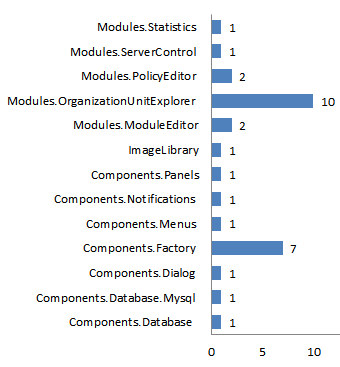
\includegraphics[scale=0.9]{pages/chapter4/figures/depth.png}
				\vspace{-6mm}
				\caption{Depth of Inheritance}
				\label{fig:DepthofInheritance}
			\end{figurehere}
			
			\begin{figurehere}
				\inputminted[linenos=true,fontsize=\footnotesize,tabsize=2,xleftmargin=1cm]{csharp}{pages/chapter4/smippets/inheritance.cs}
				\vspace{-4mm}
				\caption{Inheritance Coupling}
				\label{fig:InheritanceCoupling}
			\end{figurehere}
			
		\end{multicols}	

		\normalsize
		{
			From the two class definitions in Fig. \ref{fig:InheritanceCoupling} we can see the result of this.
			TreeViewOuElement extending from TreeViewItem introduced nine inherited dependencies 
			and the DragAdorner extending from Adorner introduced 6 dependencies inherited as part of the inheritance chain
			the Dot Net Framework.
			\newline
			\newline
			An argument for this and the reason for the intentional rule violation in terms of TreeViewOuElement is that,
			to create all the functionality of a TreeViewItem at so that it conforms or encompasses all the functionality that is
			required to realise it as a TreeViewItem, is simply too much work.  As indicated by the Dot Net Frameworks TreeViewItem
			the class is quiet complex, therefore we have to acknowledge the trade offs when deciding to re-implement the wheel
			as opposed to inheriting.  
			\newline
			\newline
			A second argument, and probably the best approach would have been to create a collection class with pair mappings
			of IOu and TreeViewItem.  As indicated by the interface realisation in \ref{fig:DepthofInheritance},  the reason
			for the inheritance was to add a member IOu and the appropriate accessor and mutator.  By creating a collection
			class with a hash table for instance, the separation of TreeViewItem \& IOu could have been achieved.  
			The appropriate accessor \& mutator could have been encapsulated by the collection class and indirection used to 
			access the appropriate pair IOu.  
			Unfortunately, this was over looked during development, but is easily fixed in future releases.
			\newline
			\newline
			NDepend gives a more in depth analysis of the application class coupling, in section. \ref{sec:SubclassesInheritance}.  
			In fact according to the NDepend qualitative definitions only the TreeViewOuElement is in violation of this rule.
		}			
			

%%%%%%%%%%%%%%%%%%%%%%%%%%%%%%%%%%%%%%%%%%%%%%%%%%%%%%%%%%%%%%%%%%%
%%%%%%%%%%%%%%%%%%%%%%%%%%%%%%%%%%%%%%%%%%%%%%%%%%%%%%%%%%%%%%%%%%%	


	\subsection{Class Coupling}		

		\vspace{-8mm}
		\textit
		{
			\begin{itemize}		
				\item \textbf{Class Coupling} 
					\begin{itemize}
						\item Measures the coupling to unique classes through parameters, local variables, return types, method calls, generic or template instantiations, base classes, interface implementations, fields defined on external types, and attribute decoration. 
						\item Good software design dictates that types and methods should have high cohesion and low coupling. 
						\item High coupling indicates a design that is difficult to reuse and maintain because of its many interdependencies on other types
					\end{itemize}
			\end{itemize}	
		} 
		-- \citet{MicroSoftMetrics} 
		\newline					

		\large{\bfseries{Interpretation}}
		\vspace{2mm}

		\normalsize
		{			
			This indicates the total number of dependencies that an item has on other types.  This number excludes primitive and built-in 
			types such as Int32, String and Object,  However does not exclude compound inbuilt types such as Button. 
			\newline
		}			
					

		\large{\bfseries{Analysis \& Improvement}}
		\vspace{2mm}
		
		\normalsize
		It is important for the reader to be aware that inbound or afferent coupling is to be observed on the Factory,
		while efferent or outbound coupling from the components.
		\newline
		\newline
			
		\begin{multicols}{2}
		
			Unfortunately visual studio does not distinguish between developer types and inbuilt .Net framework types.
			Furthermore the disbursement between Afferent Coupling (inbound) \& Efferent Coupling (outbound) and other concerns such as derived coupling,
			is not immediately indicated.  A lower value indicates the reusability of a class.
			\newline
			\newline
			From the metrics provided by NDepend in section. \ref{sec:ComplexityCoupling} a better analysis can be observed.
			There are areas from improvement and some refactoring to resolve these areas should be done in successive releases.	
			\newline
			\newline
			Areas of high coupling are indicated in red.  Once again due to the composite nature of the application; coupling
			seems rather high due to afferent and efferent coupling.  In the future releases a possible reduction
			of architectural interfaces could help to reduce the coupling.  
			
			\columnbreak
			
			\begin{figurehere}
				\centering
				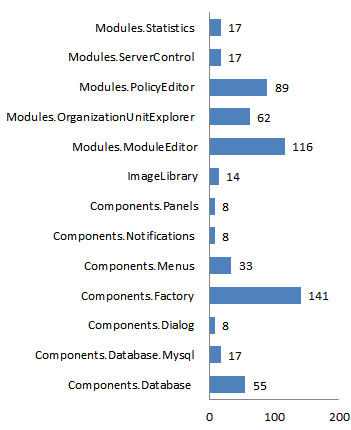
\includegraphics[scale=0.9]{pages/chapter4/figures/coupling.png}
				\vspace{-7mm}
				\caption{Class Coupling}
				\label{fig:ClassCoupling}				
			\end{figurehere}
			
		\end{multicols}
		
		\vspace{-4mm}
		\normalsize
		{				
			There are many methodologies for interface reductions such as described in A Simple Process for Specifying Component-Based Software. \citet{CheesmanDaniels}
			\newline
		}	
		
%%%%%%%%%%%%%%%%%%%%%%%%%%%%%%%%%%%%%%%%%%%%%%%%%%%%%%%%%%%%%%%%%%%
%%%%%%%%%%%%%%%%%%%%%%%%%%%%%%%%%%%%%%%%%%%%%%%%%%%%%%%%%%%%%%%%%%%	

	\subsection{Source Lines Of Code}

		\normalsize
		{
			There is are two types of SLOC measurements, physical SLOC (LOC) and logical SLOC (LLOC). 
			Specific definitions of these two measurements vary, however physical SLOC is a count of lines in the source code including comment lines.  				
			\newline
		}

		\large{\bfseries{Interpretation}}
		\vspace{2mm}
		
		\normalsize
		{
			In SLOC blank lines are also included, if blank lines exceed 25\% they are not counted toward lines of code.
			This is the simplest form of metric, this quantitative metric usually indicates the 
			scale of the project, in terms of size. 
			\newline
		}			

			
		\vspace{-7mm}
		\begin{multicols}{2}	

			\large{\bfseries{Improvement Points}}
			\vspace{2mm}
			
			\normalsize
			{
				During the calculation of these metrics the blank lines of code were left out by source monitor, contrary to the definition.  
			}			
			
			\begin{tablehere}
				\centering
				\small
				{					
					\vspace{30mm}
					\begin{tabular}{ | l | l |}
																		   \hline
						Language 					& Lines 			\\ \hline
						C\# 						& 25968(44996)		\\ \hline
						Perl 						& 7076				\\ \hline
						Xaml 						& 2353				\\ \hline
						Resx Language Translations  & 133251			\\ \hline
					\end{tabular}
				}
				\caption{SourceMonitor - Source Lines of code - SLOC}
				\label{tab:SourceMonitorLinesofcode}
			\end{tablehere}
		
		\end{multicols}
		
		\normalsize
		{	
			For the C\# analysis the larger of the two indicators 44,996, includes generated designer files generated by visual studio, but modified during development.
			There is not much we can tell from this information other than the size may indicate maintainability and understandability problems.
			\newline
		}
			

%%%%%%%%%%%%%%%%%%%%%%%%%%%%%%%%%%%%%%%%%%%%%%%%%%%%%%%%%%%%%%%%%%%
%%%%%%%%%%%%%%%%%%%%%%%%%%%%%%%%%%%%%%%%%%%%%%%%%%%%%%%%%%%%%%%%%%%	


	\subsection{Line Spread}

		\normalsize
		{
			This section shows the spread of the source code lines amongst files, the file types, classes, interfaces etc.  
			Documentation eg. (JavaDoc), comments and an introduction into the complexity of each file also.
			\newline
		}

		\vspace{-7mm}
		\begin{multicols}{2}
		
			\large{\bfseries{Interpretation}}
			\vspace{2mm}
			
			\normalsize
			{
				From this information we can now begin to see a better overview of the source code analysis.  The number of classes, interfaces and structs
				together with the number of lines per file may indicate the complexity as well as the maintainability of the source code. If the commenting and documentation 
				is at a low level understanding the code may prove difficult.  
				\newline
			}			

			\columnbreak
			
		
			\begin{tablehere}
				\centering
				\small
				{
					\begin{tabular}{ | l | l |}
																					   \hline
						Files									& 294 					\\ \hline
						lines 									& 44996					\\ \hline
						lines / file							& 153.05 				\\ \hline
						Classes, Interfaces, Structs			& 243					\\ \hline
						Methods per Class						& 6.01					\\ \hline
						Comments / file							& 7.20 					\\ \hline
						Documentation Lines / file 				& 20.26 				\\ \hline
						Maximum Cyclomatic Complexity 			& 92 					\\ \hline
						Average Cyclomatic Complexity / file	& 15.68					\\ \hline
					\end{tabular}
				}
				\caption{SourceMonitor - Line Spread}
				\label{sec:linspreadresult}	
			\end{tablehere}	
		
		\end{multicols}
				
		\large{\bfseries{Analysis}}
		\vspace{2mm}
		
		\normalsize
		{
			
			From these statistics we can ascertain that approximately 20\%(153/27) is made of documentation and commenting.				
			Typically a comment percentage less than 10 percent is considered insufficient. - (Resource Standard Metrics).
			Steve McConnell in his book \textit{Code Complete} recommends about 7 methods per class due to people being able to remember 7 items. 
			\citet{CodeComplete}.  From these statistics we comply with this recommendation. 
			\newline
			\newline
			Steve McConnell also recommends that a method should be no larger than what can be displayed on a screen - \citet{CodeComplete}.
			This makes perfect sense to me, in that a programmer does not want to be scrolling up and down as it impairs concentration.
			Taking 153 lines per document and dividing it by 6 methods, we get an average of ~25 lines.  This is very comfortably displayed and 
			leaves plenty of space to work with on a screen.
			\newline
		}	

		\large{\bfseries{Improvement}}
		\vspace{2mm}
		
		\normalsize
		{
			Even though complying with the recommendation (20\%) the spread of documentation and commenting 
			percentage results, I would have to disagree with.  The balance and quality of the commenting is more important than the amount.
			Too much commenting can make the code unreadable and as such should be clear and to the point.  
			That said more commenting(not documentation) is needed, but a focus on quality comments, not metrics.
			\newline
		}
		
				

%%%%%%%%%%%%%%%%%%%%%%%%%%%%%%%%%%%%%%%%%%%%%%%%%%%%%%%%%%%%%%%%%%%
%%%%%%%%%%%%%%%%%%%%%%%%%%%%%%%%%%%%%%%%%%%%%%%%%%%%%%%%%%%%%%%%%%%	

\newpage

	\subsection{Methods \& Statements}
	
		\vspace{-5mm}
		\begin{multicols}{2}
			
			\normalsize
			{
				In computer science statements are one of two types, simple statements such as return, method calls and assignments.
				Examples of compound statements are if, switch and while.   In this section we are primarily concerned with compound statements
				and the resulting branching or Nested Block Depth (NBD).  An example of which can be seen in Fig. \ref{fig:nesting}.
				\newline			
			}
			
			\large{\bfseries{Interpretation}}
			\vspace{2mm}
			
			\normalsize
			{
				Analysing the code and discovering the Nested Block Depth (NBD) or block level depth as seen in Fig. \ref{fig:nesting} 
				can be used as an indicator for the perceived test difficulty.
				\newline
				\newline
				A method with too much branching with many outcomes or directions can create problems when designing tests cases to
				test all the branches.  The complexity of the resulting test can be in order as complex as the method.  
				This outcome generally indicates with high probability that refactoring is needed.	
				\newline
			}	
		
			\columnbreak
		
			\begin{figurehere}
				\inputminted[linenos=true,fontsize=\footnotesize,tabsize=2,xleftmargin=1cm]{csharp}{pages/chapter4/smippets/blocks.cs}
				\vspace{-5mm}
				\caption{Statement nesting}
				\label{fig:nesting}
			\end{figurehere}
				
		\end{multicols}
						
						
		\begin{multicols}{2}
		
			\vspace{5mm}
			\large{\bfseries{Analysis}}
			\vspace{2mm}
			
			\normalsize
			{				
				With the recommended Nested Block Depth being 5 \citet{Gintenreiter}, the analysis indicates that the code is within this recommendation.
				Roughly 1\% of the code here is at block level 6.  If a block of code has over 5 nested blocks refactoring is needed. \citet{Gintenreiter}.
				\newline
				\newline
				Lines of Code at the method level is recommended to have a maximum of 50 statements - If a method has over 50 statements it is
				suggested that the method be broken up for readability and maintainability. \citet{Gintenreiter}.  Given this metric we can see that the
				analysis has on average 8.74 statements per method well within this cut off.
				\newline
				\newline
			}	
			
			\columnbreak
			
			\begin{tablehere}
				\centering
				\small
				{
					\begin{tabular}{ | l | l |}
																					   \hline
						Statements  						& 18053					\\ \hline	
						Statements / file					& 74.23 				\\ \hline	
						Calls per method 					& 1.26					\\ \hline
						Statements per Method				& 8.74					\\ \hline
						Statements at block level 0			& 22.99\%				\\ \hline
						Statements at block level 1			& 19.01\%				\\ \hline
						Statements at block level 2			& 13.42\%				\\ \hline
						Statements at block level 3			& 15.90\%				\\ \hline
						Statements at block level 4			& 12.69\%				\\ \hline
						Statements at block level 5			& 15.1\%				\\ \hline
						Statements at block level 6			& 0.89\%				\\ \hline
						Average Maximum Block Depth 		& 3.78 					\\ \hline
						Average Block Depth					& 1.53 					\\ \hline
					\end{tabular}
				}
				\caption{Methods \& Statements}
				\label{tab:MetricBreakdown2}
			\end{tablehere}	
			
		\end{multicols}	
		
		\begin{multicols}{2}
			
			\large{\bfseries{Improvement}}
			\vspace{2mm}
		
			\normalsize
			{
				A method with too many responsibilities may be difficult to understand and in general indicates refactoring is needed.
				In the book \textit{Refactoring - Improving the design of existing code} techniques such as ``inline class'' or ``replace nested condition with guard clauses'' 
				\citet{FowlerRefactoring}.
				\newline				
				\newline
				As illustrated by Fig. \ref{fig:BlocksFlowChart} ~28\% of the 
				code is at block level 4, 5 \& 6, this could be further improved by replacing blocks 4, 5 \& 6 with a
				delegated object method call or internal method call, Fig. \ref{fig:BlocksFlowChart}.  
			}	

			\columnbreak			

			\begin{figurehere}
				\centering
				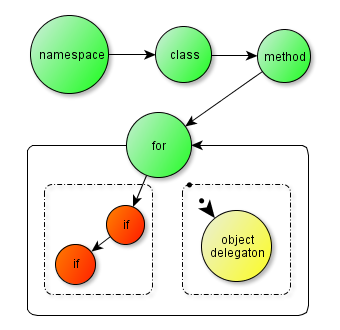
\includegraphics[scale=0.6]{pages/chapter4/figures/blocks.png}
				\vspace{-2mm}
				\caption{Block level flow chart}
				\label{fig:BlocksFlowChart}
			\end{figurehere}
		
		\end{multicols}
		
		\normalsize
		{
			Even though the metrics are in line with \citet{Gintenreiter}'s
			research on static analysis and metrics; by analysing the final two metrics Average Maximum Block Depth (3.78) and
			Average Block Depth (1.53 ) it may be possible to refactor the implementation further.
			By negating blocks 4,5,6 as much as possible, the average maximum block depth and resulting overall average could be reduced making it easier
			to manage, debug, test etc.
			\newline
		}	
				

%%%%%%%%%%%%%%%%%%%%%%%%%%%%%%%%%%%%%%%%%%%%%%%%%%%%%%%%%%%%%%%%%%%
%%%%%%%%%%%%%%%%%%%%%%%%%%%%%%%%%%%%%%%%%%%%%%%%%%%%%%%%%%%%%%%%%%%	


	\subsection{Metrics Overview}

		An overall summary of the maintainability, cyclomatic complexity, depth of inheritance and class coupling as provided by visual studio.
				
		\begin{figure}[h!]
		\centering
		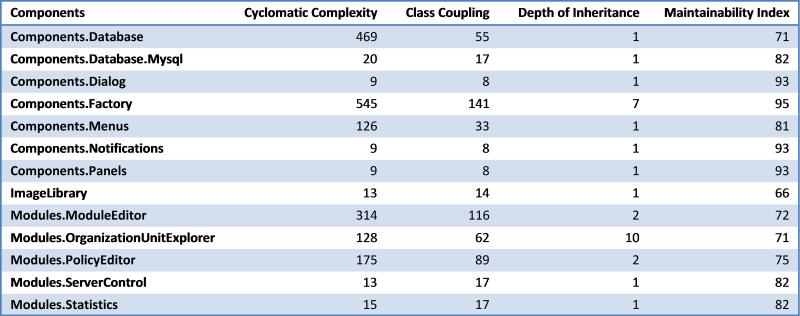
\includegraphics[scale=0.75]{pages/chapter4/figures/4metrics.png}
		\caption{Visual Studio Metrics Overview}
		\label{fig:VisualStudioMetricsOverview}
		\end{figure}			

	\vspace{-3mm}
	\subsection{Code Coverage}

		\normalsize
		{
			Considering the quantity of code involved and the time frame available, the exploratory
			testing achieved a reasonable coverage analysis as illustrated in Figure \ref{fig:MetricCodeCoverageAnalysis}.
			It's important to point out that during the tests, the majority of exploratory paths were attempted and the large percentage
			of the untested code is exception handling or non used interface methods that are realised by classes. 		
		}

		\begin{figure}[h!]
			\centering
			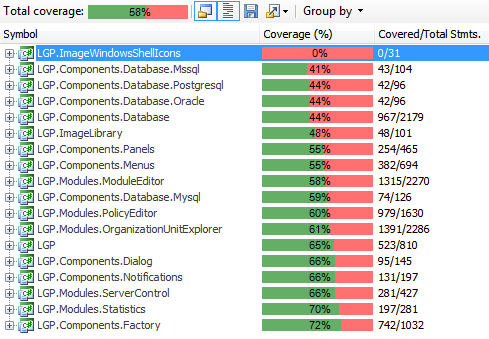
\includegraphics[scale=0.9]{pages/chapter4/figures/coverage-overview.png}
			\vspace{-3mm}
			\caption{Code Coverage Overview}
			\label{fig:MetricCoverageOverview}
		\end{figure}

		\normalsize
		{
			Empirical studies pointed out the Bullseye Software Testing Group of real projects found that increasing code coverage above 70-80\% is 
			time consuming and not cost effective - \citet{SteveCornett}. The Risk assessment of a project should be ascertained, for instance aviation requires 100\% coverage.  
			As this is not a high risk product and people are not going to die (my supervisor suggested I personalise this a little), 
			100\% code coverage is not required. 
			\newline
		}
		
		\vspace{-3mm}
		\normalsize
		{
			Bullseye also go onto say 100\% code coverage is estimated to expose 50\% of the bugs, low code coverage indicates inadequate testing and high code coverage 
			guarantees nothing - \citet{SteveCornett}.  Bullseye and other static code analysis investors generally point towards the 90, 80, 70 rule of, 90\% unit testing, 
			80\% integration testing, and 70\% system testing. \citet{SteveCornett}
			\newline
		}
		
		\vspace{-3mm}
		\normalsize
		{
			While it's not indicated in the post coverage analysis, a large proportion of the indicated untested code was tested 
			during unit testing, in the development phase.  During development better defensive programming was introduced on the discovery of bugs.
			As each successive bug was negated via better inspection (if-else) the quality improved.
			The testing of else blocks or catch blocks became increasingly more difficult to test and as indicated by the analysis.	
		}

		\begin{figure}[h!]
			\centering
			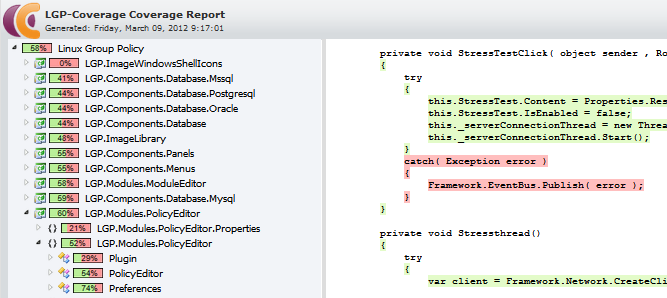
\includegraphics[scale=0.8]{pages/chapter4/figures/coverage-snippet.png}
			\vspace{-2mm}
			\caption{Code Coverage Analysis}
			\label{fig:MetricCodeCoverageAnalysis}
		\end{figure}

